\documentclass[a4paper, 12pt]{article}

%%%%%%%%%%%%%%%%%%%%%%%%%%%%%%% PACKAGES %%%%%%%%%%%%%%%%%%%%%%%%%%%%%%%
% Math-related things
\usepackage{amsmath}
\usepackage{amssymb}
\usepackage{amsthm}
% Italian spelling
\usepackage[italian]{babel}
% Accenti e caratteri speciali
\usepackage[utf8]{inputenc}
% Margini e grafica della pagina
\usepackage[top=2cm, bottom=2cm, left=2cm, right=2cm]{geometry}
\usepackage{fancyhdr}
% Tabelle
\usepackage{tabularx}
% Graphs and Images handling
\usepackage{graphicx}
\usepackage{svg}
% Programming languages support
\usepackage{minted}
% Hypertext references
\usepackage{hyperref}
% Citations
\usepackage{epigraph}

% Title Page
\title{TasteIt - Progetto di Ingegneria Informatica}
\author{
	Paolo Pertino [10729600]
	\href{mailto:paolo.pertino@mail.polimi.it}{paolo.pertino@mail.polimi.it} \\
} 

% Contents page settings
\renewcommand*\contentsname{Indice}
\setcounter{tocdepth}{3}

\newcommand{\quantities}[1]{%
	\begin{tabular}{@{}c@{}}\strut#1\strut\end{tabular}%
}

% General page settings
\pagestyle{fancy}
\fancyhf{}
\rhead{\leftmark}
\lhead{TasteIt - Progetto di Ingegneria Informatica}
\cfoot{\thepage}

% Hyperrefs setup
\hypersetup{
	colorlinks=true,
	linkcolor=[rgb]{0.996,0.396,0.090196}, %254 101 23
	filecolor=magenta,      
	urlcolor=[rgb]{0.72156862745,0.0078431372549,0.00392156862745},
	citecolor=[rgb]{0.517647,0.0156862745,0.0117647},
	pdftitle={TasteIt - Progetto di Ingegneria Informatica},
	pdfpagemode=FullScreen,
}

\begin{document}
	\pagenumbering{gobble}
	\date{\today}
	\maketitle
	
	\begin{figure}[h!]
		\centering
		\includegraphics[scale=0.35]{tasteitIntro.png}
	\end{figure}

	\newpage
	\pagenumbering{arabic}
	
	\tableofcontents
	
	\newpage
	
	\section{Introduzione}
	\paragraph{}
	TasteIt è un bot Telegram che si propone di aiutare gli utenti a effettuare una ricerca del ristorante in cui consumare un pasto, in base alle loro esigenze in termini di ciò che vogliono consumare, di orario e di prezzo. La ricerca può aver inizio a partire dalla propria posizione, oppure dal nome di una località, piazza o via di interesse.\\
	Infine, la semplice operazione di ricerca è stata corredata dalla possibilità di creare liste dei preferiti, interattività della conversazione nei gruppi con possibilità di creare sondaggi ed è inoltre fornito un supporto per diverse lingue (attualmente sono implementate solo Italiano e Inglese).
	
	\subsection{Installazione}
	\paragraph{}
	Per poter avviare il bot è necessario avere Python 3.x \cite{python_installation} installato sul proprio dispositivo.\\
	Attraverso il packet manager \textit{pip} installare i requirements elencati nel file \textit{requirements.txt}, recandosi nella directory principale del progetto (\textit{./TasteIt}) e digitando il comando:
	\begin{minted}{bash}
		$ pip install -r requirements.txt
	\end{minted}
\subsubsection{Configurazione Telegram}
	\paragraph{}
	Successivamente è necessario creare un bot attraverso \textit{@BotFather} ed ottenere la API key associata \cite{telegram_bot_creation}.\\
	Creare dunque un file \textit{.env} all'interno della cartella \textit{/src} in cui inserire la chiave appena generata con il seguente formato:
	\begin{minted}{bash}
		TELEGRAM_KEY=la_tua_chiave
	\end{minted}
	\paragraph{}
	Inoltre, collegarsi nella chat di \textit{@chatIDrobot} e premere \textit{Avvia} per ottenere informazioni riguardanti la propria chat. Copiare il numero che segue la dicitura \textit{chat\_id} ed inserirlo nel file \textit{.env} con il formato seguente:
	\begin{minted}{bash}
		TELEGRAM_DEVELOPER_CHAT_ID_KEY=chat_id_copiato
	\end{minted}
	In questo modo quando un errore inaspettato verrà riscontrato da un utente, il bot provvederà in automatico a segnalare lo sviluppatore.
	\paragraph{}
	La configurazione dei parametri inerenti Telegram è ora completata.
	
	\subsubsection{Configurazione Google}
	\paragraph{}
	Infine, siccome il funzionamento del bot è relegato all'utilizzo dei servizi offerti da Google, attraverso le \textit{Places API}, è necessario registrare un account su \textit{Google Cloud Services} e fare richiesta per l'abilitazione di una key per le suddette API \cite{places_api_key_registration}.
	Una volta ottenuta le chiave, inserirla all'interno del file \textit{.env} con il formato che segue:
	\begin{minted}{bash}
		GOOGLE_PLACES_KEY=la_tua_google_api_key
	\end{minted}
	\paragraph{}
	Terminato questo passaggio, il bot è pronto per essere avviato. Digitare dunque il comando:
	\begin{minted}{bash}
		$ py ./main.py
	\end{minted}
	per avviare l'applicativo.
	
	\newpage
	% Lista di funzionalità
	\section{Funzionalità TasteIt}
	Di seguito elenchiamo le funzionalità offerte dal bot ed i comandi necessari per l'interazine.
	\begin{itemize}
		\item \textit{/start} - Avvia il bot mostrando un messaggio di benvenuto all'utente.
		\item \textit{/lang} - Permette il cambio di lingua. Esso impatterà sia sui messaggi di servizio sia sugli effettivi risultati di ricerca.
		\item \textit{/cerca} - Introduce la conversazione per iniziare la ricerca di un ristorante.
		\item \textit{/preferiti} - Mostra all'utente (o al gruppo) le sue liste preferiti.
		\item \textit{/annulla} - Annulla l'operazione corrente.
	\end{itemize}
	
	\subsection{/lang - Modifica lingua}
	Digitando il comando \textit{/lang} è possibile modificare la lingua con cui interagire con il bot. Quest'ultimo invierà un messaggio con allegato una tastiera contenente le lingue disponibili (di default soltanto Italiano ed Inglese).
	
	\begin{figure}[h!]
		\centering
		\includegraphics[scale=1.1]{langCommand.png}
		\caption{Risposta al comando /lang}
	\end{figure}

	Selezionando una delle bandiere, la lingua muterà in quella selezionata ed i dati verranno anche aggiornati nel database.
	
	\subsection{/cerca - Ricerca dei ristoranti}
	TODO: Inserire ricerca ristoranti
	
	\subsection{/preferiti - Lista dei preferiti}
	TODO: Inserire lista dei preferiti
	
	\newpage
	% Architettura
	\section{Architettura}
	Nella sezione corrente viene resa esplicita l'architettura dell'applicativo. Nello specifico vengono presentate ed analizzate:
	\begin{itemize}
		\item Struttura del database.
		\item Oggetti custom creati per gestire le liste di ristoranti.
		\item Macchine a stati rappresentanti le conversazioni.
	\end{itemize}
	\subsection{Database}
	Nella Figura \ref{fig:ER_image} è stato riportato il diagramma ER rappresentante la semplice struttura del database.
	\begin{figure}[h!]
		\centering
		\includegraphics[scale=0.7]{tasteItDb.png}
		\caption{Schema ER Database TasteIt}
		\label{fig:ER_image}
	\end{figure}
	\paragraph{}
	La relazione \textit{'Contiene'} è stata successivamente trasformata in una tabella ponte chiamata \textit{restaurant\_for\_list}.
	Pertanto, riportiamo di seguito lo schema logico dedotto dalla progettazione concettuale effettuata.\\
	chat(\textbf{chat\_id}, lang)\\
	restaurant(\textbf{restaurant\_id}, name, address, phone\_number, rating, website, total\_ratings, price\_lvl, timetable, maps\_link)\\
	list(\textbf{list\_id}, category, chat\_id)\\
	restaurant\_for\_list(\textbf{list\_id, chat\_id})\\
	list.chat\_id $\rightarrow$ chat.chat\_id\\
	restaurant\_for\_list.list\_id $\rightarrow$ list.list\_id\\
	restaurant\_for\_list.chat\_id $\rightarrow$ chat.chat\_id
	
	\subsection{Class Diagram}
	\paragraph{}
	Di seguito riportiamo inoltre un class diagram degli oggetti ausiliari creati ed utilizzati ai fini del progetto.\\
	\begin{figure}[h]
		\centering
		\def\svgwidth{\columnwidth}
		\resizebox{\linewidth}{!}{\input{{tasteit_class_diagram.pdf_tex}}}
		\caption{TasteIt - Class Diagram}
		\label{fig:class_diagram}
	\end{figure}
	\paragraph{}
	Segue una breve descrizione del contenuto della Figura \ref{fig:class_diagram}:
	\begin{itemize}
		\item \textit{Service} enumerazione rappresentante i servizi per cui è disponibile una API key;
		\item \textit{ApiKey} rappresenta la chiave stessa. Il metodo \textit{value} cerca la key del servizio specificato all'interno del file \textit{.env} o tra le variabili d'ambiente del sistema;
		\item \textit{ResearchInfo} rappresenta le informazioni preliminari utili per effettuare una ricerca di un ristorante;
		\item \textit{GeneralPlace} contiene le informazioni relative alla posizione di un determinato luogo;
		\item \textit{DoublyCircularArrayList} classe astratta rappresentante una doppia lista circolare\cite{circularDoublyLinkedList} (differente dalla versione linked, in quanto i nodi non sono effettivamente linkati tra loro);
		\item \textit{Restaurant} rappresenta un ristorante e tutte le sue informazioni (nome, latitudine, longitudine, 'costosità', valutazione media degli utenti, numero totale di recensioni, orario settimanale, indirizzo, sito web, link a google maps e numero di telefono);
		\item \textit{Rating} rappresenta una recensione (autore, valutazione, contenuto e data);
		\item \textit{RestaurantsList} implementazione di DoublyCircularArrayList rappresentante una lista di ristoranti;
		\item \textit{RatingsList} implementazione di DoublyCircularArrayList rappresentante una lista di recensioni;
		\item \textit{ListIterator} iteratore per le liste sopra descritte, il quale le rende iterabili da inizio a fine;
		\item \textit{FavoriteList} rappresenta una lista preferiti (id, categoria e ristoranti in essa contenuti);
	\end{itemize}

	\subsection{Conversazioni - Macchine a stati}
	\paragraph{}
	In questa sezione verranno presentate le macchine a stati schematizzanti le conversazioni offerte dal bot e gli eventi che scatenano i cambiamenti di stato.
	\subsubsection{Modifica della lingua}
	\paragraph{}
	La conversazione più semplice: in risposta al comando \textit{/lang} viene invocata la funzione \textit{setLanguage()} che presenta all'utente il messaggio con la tastiera per scegliere la lingua da utilizzare.\\
	\begin{figure}[h!]
		\centering
		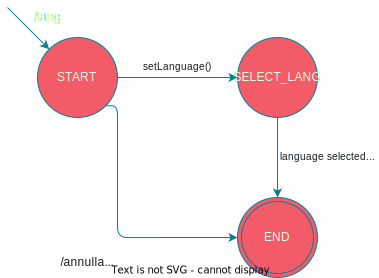
\includegraphics[scale=0.7]{TasteIt_Lang_StateMachine.png}
		\caption{/lang - State Machine}
		\label{fig:LangStateMachine}
	\end{figure}
	
	\newpage
	\subsubsection{Ricerca ristorante}
	\paragraph{}
	Risponde alla richiesta effettuata con il comando \textit{/cerca} e gestisce l'intera conversazione di ricerca dei ristoranti e visualizzazione dei risultati.\\
	\begin{figure}[h!]
	\centering
	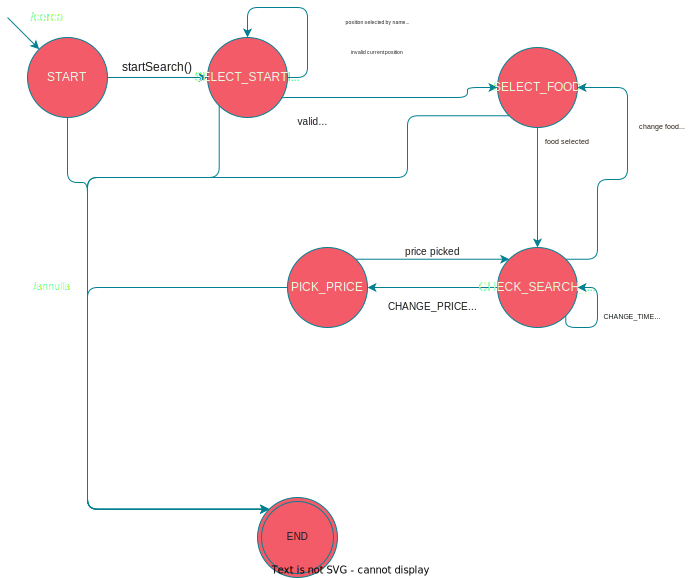
\includegraphics[scale=0.7]{TasteIt_Cerca_StateMachine.png}
	\caption{/cerca - State Machine}
	\label{fig:CercaStateMachine}
	\end{figure}
	
	% Strumenti usati
	\newpage
	\section{Strumenti utilizzati}
	Nella seguente sezione verranno indicati i principali strumenti di sviluppo utilizzati:\\
	\begin{itemize}
		\setlength{\parskip}{0pt}
		\setlength{\parsep}{0pt}
		
		\item \emph{Visual Studio Code} - Principale IDE utilizzato.
		\item \emph{python-telegram-bot} - Wrapper python usato per interfacciarsi con le API di Telegram.
		\item \emph{Places API} - Google Maps API; gestiscono l'operazione di ricerca dei ristoranti.
		\item \emph{SQLite3} - modulo per interagire con le API dell'omonima libreria SQLite, utilizzata per creare e gestire databases in locale.
		\item \emph{Raspberry PI 4} - Hosting del bot e gestione del database.
		\item \emph{AstahUML} - Creazione di diagrammi UML.
		\item \emph{GitKraken} - Git GUI per visualizzare il workflow di sviluppo ed utilizzare efficientemente Git.
		\item \emph{TEXStudio} - Gestione e aggiornamento del report.
	\end{itemize}
	% Bibliografia
	\newpage
	\begin{thebibliography}{99}
		\bibitem{python_installation}
		\href{https://www.python.org/downloads/}{Python Download \& Installation}
		
		\bibitem{telegram_bot_creation}
		\href{https://sendpulse.com/knowledge-base/chatbot/create-telegram-chatbot}{Create a Telegram bot}
		
		\bibitem{places_api_key_registration}
		\href{https://developers.google.com/maps/documentation/places/web-service/get-api-key}{Google Cloud Platform - Places API Key}
		
		\bibitem{circularDoublyLinkedList}
		\href{https://pythonwife.com/circular-doubly-linked-list-in-python/#:~:text=A%20circular%20doubly%20linked%20list,tail%20node%20and%20vice%20versa.}{Circular Doubly Linked List}
		
	\end{thebibliography} 
\end{document}         
